% opposition-agents-playing-mtg --- Full Project Overview
% Compile: pdflatex full_project_overview.tex (twice for ToC)

\documentclass[aspectratio=169, 10pt]{beamer}

% --- Theme ---------------------------------------------------------
\usetheme{Madrid}
\usecolortheme{seahorse}
\setbeamertemplate{navigation symbols}{}
\setbeamertemplate{footline}[frame number]
\setbeamertemplate{itemize items}[circle]

% --- Packages ------------------------------------------------------
\usepackage{tikz}
\usetikzlibrary{
  positioning, arrows.meta, shapes.geometric, fit, calc,
  backgrounds, decorations.pathreplacing, matrix
}
\usepackage{booktabs}
\usepackage{amsmath, amssymb}
\usepackage{listings}
\usepackage{xcolor}
\usepackage{multicol}

% --- Colors --------------------------------------------------------
\definecolor{mtgblue}{HTML}{1E3A5F}
\definecolor{mtgred}{HTML}{C13A28}
\definecolor{mtggreen}{HTML}{2D6A2E}
\definecolor{mtggold}{HTML}{D4A843}
\definecolor{kgpurple}{HTML}{6B3FA0}
\definecolor{jepaorange}{HTML}{E07020}
\definecolor{codebg}{HTML}{F5F5F0}
\definecolor{lgray}{HTML}{E8E8E8}

% --- Listings ------------------------------------------------------
\lstset{
  basicstyle=\ttfamily\tiny,
  backgroundcolor=\color{codebg},
  frame=single,
  rulecolor=\color{lgray},
  breaklines=true,
  columns=fullflexible,
  keywordstyle=\color{mtgblue}\bfseries,
  commentstyle=\color{mtggreen},
  stringstyle=\color{mtgred},
}

% --- Metadata ------------------------------------------------------
\title[Opposition Agents Playing MTG]{%
  Opposition Agents Playing\\Magic: The Gathering}
\subtitle{Knowledge Graphs, World Models, JEPA, and Active Inference\\
  for the Hardest Popular Game in AI}
\author{Felix Neuburger}
\date{2025}

% ===================================================================
\begin{document}

% --- Title ---------------------------------------------------------
\begin{frame}
  \titlepage
\end{frame}

% --- Outline -------------------------------------------------------
\begin{frame}{Outline}
  \tableofcontents
\end{frame}


% ===================================================================
\section{Introduction}
% ===================================================================

% --- Slide: Problem Statement --------------------------------------
\begin{frame}{Why Magic: The Gathering?}
  \begin{center}
    \large\bfseries The hardest popular card game for AI.
  \end{center}
  \vspace{0.3cm}
  \begin{center}
  \begin{tabular}{@{}lcccc@{}}
    \toprule
    \textbf{Dimension} & \textbf{Chess} & \textbf{Go} & \textbf{Poker} & \textbf{MTG} \\
    \midrule
    State space         & $\sim10^{47}$  & $\sim10^{170}$ & $\sim10^{6}$   & $\mathbf{\sim10^{800+}}$ \\
    Unique pieces/cards & 6              & 1               & 52             & \textbf{28,000+} \\
    Hidden information  & None           & None            & 2 cards        & \textbf{50--90 cards} \\
    Action space (avg)  & $\sim$30       & $\sim$250       & $\sim$5        & \textbf{0--100+} \\
    Rule complexity     & $\sim$50 pp    & $\sim$20 pp     & $\sim$5 pp     & \textbf{$\sim$260 pp} \\
    \bottomrule
  \end{tabular}
  \end{center}
  \vspace{0.2cm}
  \begin{center}
    \footnotesize
    Chess fell to tree search. Go fell to neural MCTS. Poker fell to CFR.\\
    \textbf{MTG hasn't fallen to anything.}
  \end{center}
\end{frame}

% --- Slide: Project Goals ------------------------------------------
\begin{frame}{Project Goals}
  Build a \textbf{complete research framework} --- not a toy prototype.
  \vspace{0.3cm}
  \begin{columns}[T]
    \begin{column}{0.48\textwidth}
      \textbf{AI research:}
      \begin{itemize}\small
        \item Planning under uncertainty in large POMDPs
        \item Zero-shot generalization to new cards
        \item Opponent modeling with hidden state
        \item Structured reasoning over complex rules
        \item Self-play with dream-based RL
      \end{itemize}
    \end{column}
    \begin{column}{0.48\textwidth}
      \textbf{Engineering:}
      \begin{itemize}\small
        \item Python-native game engine ($>$1000 games/hr)
        \item 7 agent architectures---plug-and-play
        \item Neo4j Knowledge Graph (28K+ cards)
        \item V+M+C world model with JEPA
        \item Docker deployment with GPU support
      \end{itemize}
    \end{column}
  \end{columns}
  \vspace{0.4cm}
  \begin{center}
    \footnotesize
    Targets Standard (1v1, 20 life) and Commander/EDH (4-player, 40 life).\\
    \textbf{Transfer learning curriculum:} Standard $\to$ Commander.\\
    Python 3.11+, MIT License.
  \end{center}
\end{frame}


% ===================================================================
\section{Architecture}
% ===================================================================

% --- Slide: 6-Layer Stack ------------------------------------------
\begin{frame}[fragile]{System Architecture: 6-Layer Stack}
  \begin{center}
  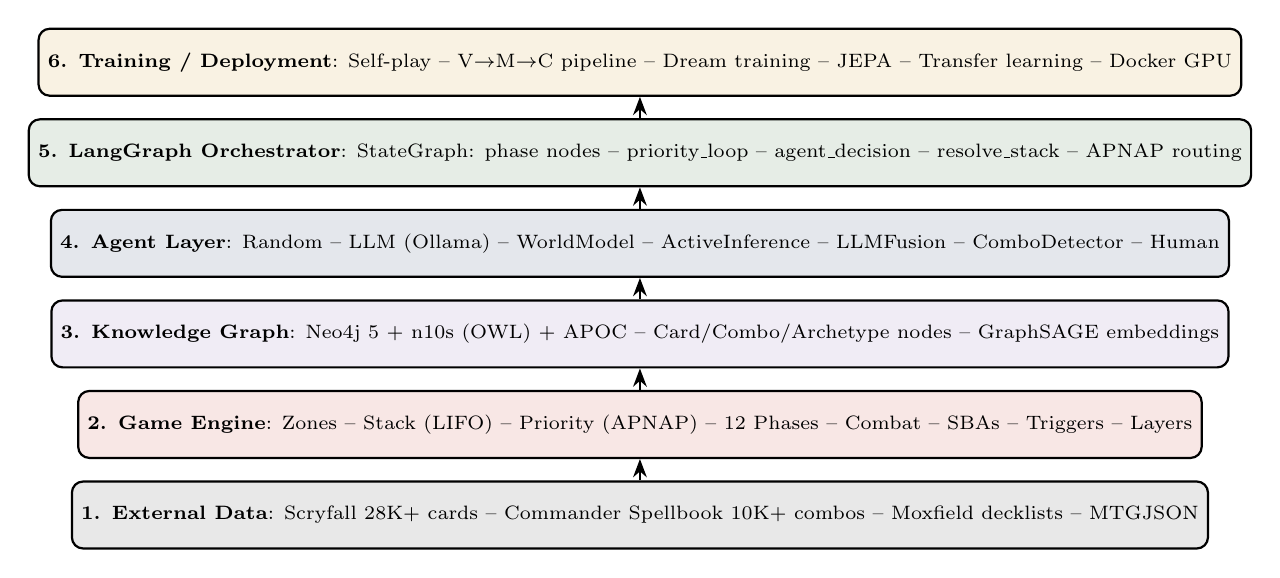
\begin{tikzpicture}[
      every node/.style={font=\scriptsize},
      layer/.style={draw, thick, rounded corners, fill=#1,
                    minimum width=12cm, minimum height=0.85cm, align=center},
      >=Stealth,
    ]
    \node[layer=lgray]          (L1) at (0, 0)
      {\textbf{1. External Data}: Scryfall 28K+ cards -- Commander Spellbook 10K+ combos -- Moxfield decklists -- MTGJSON};
    \node[layer=mtgred!12]      (L2) at (0, 1.15)
      {\textbf{2. Game Engine}: Zones -- Stack (LIFO) -- Priority (APNAP) -- 12 Phases -- Combat -- SBAs -- Triggers -- Layers};
    \node[layer=kgpurple!10]    (L3) at (0, 2.30)
      {\textbf{3. Knowledge Graph}: Neo4j 5 + n10s (OWL) + APOC -- Card/Combo/Archetype nodes -- GraphSAGE embeddings};
    \node[layer=mtgblue!12]     (L4) at (0, 3.45)
      {\textbf{4. Agent Layer}: Random -- LLM (Ollama) -- WorldModel -- ActiveInference -- LLMFusion -- ComboDetector -- Human};
    \node[layer=mtggreen!12]    (L5) at (0, 4.60)
      {\textbf{5. LangGraph Orchestrator}: StateGraph: phase nodes -- priority\_loop -- agent\_decision -- resolve\_stack -- APNAP routing};
    \node[layer=mtggold!15]     (L6) at (0, 5.75)
      {\textbf{6. Training / Deployment}: Self-play -- V$\to$M$\to$C pipeline -- Dream training -- JEPA -- Transfer learning -- Docker GPU};

    \draw[->, thick] (L1.north) -- (L2.south);
    \draw[->, thick] (L2.north) -- (L3.south);
    \draw[->, thick] (L3.north) -- (L4.south);
    \draw[->, thick] (L4.north) -- (L5.south);
    \draw[->, thick] (L5.north) -- (L6.south);
  \end{tikzpicture}
  \end{center}
\end{frame}

% --- Slide: Data Flow Diagram -------------------------------------
\begin{frame}{Data Flow: State $\to$ Action}
  \begin{center}
  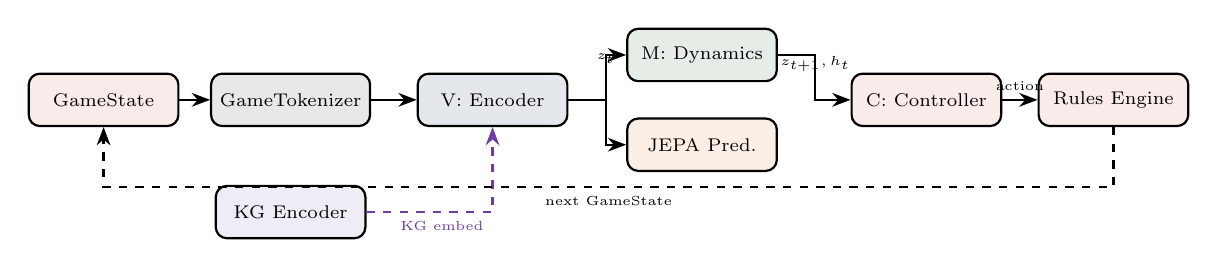
\begin{tikzpicture}[
      every node/.style={font=\scriptsize},
      block/.style={draw, rounded corners, minimum width=2cm, 
                    minimum height=0.7cm, align=center, thick},
      >=Stealth, scale=0.95, transform shape,
    ]
    \node[block, fill=mtgred!10]    (gs)  at (0, 0)     {GameState};
    \node[block, fill=lgray]        (tok) at (2.5, 0)   {GameTokenizer};
    \node[block, fill=mtgblue!12]   (V)   at (5.2, 0)   {V: Encoder};
    \node[block, fill=mtggreen!12]  (M)   at (8, 0.6)   {M: Dynamics};
    \node[block, fill=jepaorange!12](J)   at (8, -0.6)  {JEPA Pred.};
    \node[block, fill=mtgred!10]    (C)   at (11, 0)    {C: Controller};
    \node[block, fill=mtgred!10]    (re)  at (13.5, 0)  {Rules Engine};

    \node[block, fill=kgpurple!10]  (kg)  at (2.5, -1.5){KG Encoder};

    \draw[->, thick] (gs) -- (tok);
    \draw[->, thick] (tok) -- (V);
    \draw[->, thick] (V.east) -- ++(0.5,0) |- (M.west)
      node[pos=0.3, above, font=\tiny] {$z_t$};
    \draw[->, thick] (V.east) -- ++(0.5,0) |- (J.west);
    \draw[->, thick] (M.east) -- ++(0.5,0) |- (C.west)
      node[pos=0.3, above, font=\tiny] {$z_{t+1}, h_t$};
    \draw[->, thick] (C) -- (re)
      node[midway, above, font=\tiny] {action};
    \draw[->, thick, dashed, kgpurple] (kg) -| (V)
      node[pos=0.3, below, font=\tiny] {KG embed};

    \draw[->, thick, dashed] (re.south) -- ++(0,-0.8) -| (gs.south)
      node[pos=0.25, below, font=\tiny] {next GameState};
  \end{tikzpicture}
  \end{center}
  \vspace{0.2cm}
  \begin{center}
  \footnotesize
  \begin{tabular}{@{}ll@{}}
    GameState $\to$ GameTokenizer: & structured features $\to$ tensors (12 + 12 + 10$\times$128 + 20$\times$128 + \ldots) \\
    V: StateEncoder (VAE):         & features $\to$ $z \in \mathbb{R}^{256}$, optional KG residual fusion \\
    M: MDN-LSTM / JEPA:            & $z_t, a_t \to z_{t+1}$ (5-component Gaussian mixture or Transformer) \\
    C: Controller:                 & $z, h \to$ action index ($\sim$104K params, CMA-ES or PG)
  \end{tabular}
  \end{center}
\end{frame}

% --- Slide: Repository Structure -----------------------------------
\begin{frame}{Repository Map}
  \begin{columns}[T]
    \begin{column}{0.31\textwidth}
      \footnotesize
      \textbf{src/engine/}\\
      \begin{itemize}\scriptsize
        \item game\_simulator.py
        \item game\_execution.py
        \item combat.py
        \item abilities.py
        \item continuous\_effects.py
        \item card\_database.py
        \item game\_logger.py
      \end{itemize}
      \vspace{0.15cm}
      \textbf{src/agents/}\\
      \begin{itemize}\scriptsize
        \item base\_agent.py
        \item random, llm, world\_model
        \item active\_inference.py
        \item combo\_detector.py
        \item opponent\_model.py
        \item llm\_fusion\_agent.py
      \end{itemize}
    \end{column}
    \begin{column}{0.31\textwidth}
      \footnotesize
      \textbf{src/world\_model/}\\
      \begin{itemize}\scriptsize
        \item state\_encoder.py (V)
        \item dynamics\_model.py (M)
        \item controller.py (C)
        \item world\_model.py
        \item jepa\_predictor.py
        \item kg\_encoder.py
        \item game\_tokenizer.py
        \item card\_embeddings.py
      \end{itemize}
      \vspace{0.15cm}
      \textbf{src/training/}\\
      \begin{itemize}\scriptsize
        \item rl\_trainer.py
        \item self\_play.py
        \item dream\_trainer.py
        \item transfer\_learning.py
      \end{itemize}
    \end{column}
    \begin{column}{0.31\textwidth}
      \footnotesize
      \textbf{src/knowledge/}\\
      \begin{itemize}\scriptsize
        \item knowledge\_graph.py
        \item graph\_embedder.py
        \item graph\_rag.py
        \item ontology\_manager.py
      \end{itemize}
      \vspace{0.15cm}
      \textbf{data/ontology/}\\
      \begin{itemize}\scriptsize
        \item mtg-ontology-v1.1.owl
        \item mtg-shapes.ttl
      \end{itemize}
      \vspace{0.15cm}
      \textbf{scripts/}\\
      \begin{itemize}\scriptsize
        \item import\_scryfall.py
        \item import\_combos.py
        \item build\_embeddings.py
        \item train\_pipeline.py
        \item deploy.py
      \end{itemize}
    \end{column}
  \end{columns}
\end{frame}


% ===================================================================
\section{Game Engine}
% ===================================================================

% --- Slide: Engine Overview ----------------------------------------
\begin{frame}[fragile]{Game Engine: Pure-Python, RL-Ready}
  Existing engines (XMage, Forge) are Java, UI-coupled, no RL API.\\
  We built a pure-functional Python engine returning new \texttt{GameState} per action.
  \vspace{0.2cm}
  \begin{columns}[T]
    \begin{column}{0.48\textwidth}
      \begin{lstlisting}[language=Python]
state = GameState(players, decks)
while not state.game_over:
    actions = get_legal_actions(state)
    choice = agent.choose_action(
        state, actions)
    state = execute_action(state, choice)
      \end{lstlisting}
      \vspace{0.1cm}
      \footnotesize
      \textbf{Immutable transitions} $\Rightarrow$ safe for MCTS branching.\\
      \textbf{get\_legal\_actions()} $\Rightarrow$ indexed, maskable.\\
      \textbf{$>$1000 games/hour} simulation throughput.
    \end{column}
    \begin{column}{0.48\textwidth}
      \footnotesize
      \textbf{Core classes:}
      \begin{itemize}\scriptsize
        \item \texttt{GameState}: game\_id, phase, players[], cards[], stack[], combat, turn, winner
        \item \texttt{PlayerState}: life, mana\_pool \{W,U,B,R,G,C\}, commander\_tax, land\_plays
        \item \texttt{CardInstance}: UUID, card\_data, zone, owner, controller, tapped, counters, damage
        \item \texttt{Action}: type, player\_id, card\_id
        \item \texttt{ActionType}: CAST\_SPELL, PLAY\_LAND, DECLARE\_ATTACKERS, DECLARE\_BLOCKERS, ACTIVATE\_ABILITY, PASS\_PRIORITY
      \end{itemize}
    \end{column}
  \end{columns}
\end{frame}

% --- Slide: Phases & Priority --------------------------------------
\begin{frame}{Turn Structure: 12 Phases + APNAP Priority}
  \begin{center}
  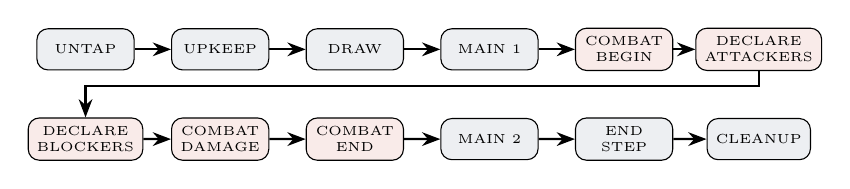
\begin{tikzpicture}[
      every node/.style={font=\tiny},
      phase/.style={draw, rounded corners, fill=mtgblue!8,
                    minimum width=1.3cm, minimum height=0.55cm, align=center},
      combphase/.style={draw, rounded corners, fill=mtgred!10,
                        minimum width=1.3cm, minimum height=0.55cm, align=center},
      >=Stealth, scale=0.95, transform shape,
    ]
    % Row 1
    \node[phase] (p1) at (0,0)     {UNTAP};
    \node[phase] (p2) at (1.8,0)   {UPKEEP};
    \node[phase] (p3) at (3.6,0)   {DRAW};
    \node[phase] (p4) at (5.4,0)   {MAIN 1};
    \node[combphase] (p5) at (7.2,0)   {COMBAT\\BEGIN};
    \node[combphase] (p6) at (9.0,0)   {DECLARE\\ATTACKERS};
    % Row 2
    \node[combphase] (p7)  at (0,-1.2)   {DECLARE\\BLOCKERS};
    \node[combphase] (p8)  at (1.8,-1.2) {COMBAT\\DAMAGE};
    \node[combphase] (p9)  at (3.6,-1.2) {COMBAT\\END};
    \node[phase] (p10) at (5.4,-1.2) {MAIN 2};
    \node[phase] (p11) at (7.2,-1.2) {END\\STEP};
    \node[phase] (p12) at (9.0,-1.2) {CLEANUP};

    \draw[->, thick] (p1) -- (p2);
    \draw[->, thick] (p2) -- (p3);
    \draw[->, thick] (p3) -- (p4);
    \draw[->, thick] (p4) -- (p5);
    \draw[->, thick] (p5) -- (p6);
    \draw[->, thick] (p6.south) -- ++(0,-0.2) -| (p7.north);
    \draw[->, thick] (p7) -- (p8);
    \draw[->, thick] (p8) -- (p9);
    \draw[->, thick] (p9) -- (p10);
    \draw[->, thick] (p10) -- (p11);
    \draw[->, thick] (p11) -- (p12);
  \end{tikzpicture}
  \end{center}
  \vspace{0.3cm}
  \begin{columns}[T]
    \begin{column}{0.48\textwidth}
      \footnotesize
      \textbf{Priority system (APNAP):}
      \begin{itemize}\scriptsize
        \item Active player gets priority first
        \item Each player may act or pass
        \item All pass + stack non-empty $\to$ resolve top
        \item All pass + stack empty $\to$ advance phase
        \item Instants/abilities can be cast anytime with priority
      \end{itemize}
    \end{column}
    \begin{column}{0.48\textwidth}
      \footnotesize
      \textbf{State-Based Actions (CR 704):}
      \begin{itemize}\scriptsize
        \item 0 life $\to$ player loses
        \item 0 toughness $\to$ creature dies
        \item Legend rule enforcement
        \item Lethal damage $\to$ destroy
        \item Checked before each priority grant
      \end{itemize}
    \end{column}
  \end{columns}
\end{frame}

% --- Slide: Zones --------------------------------------------------
\begin{frame}[fragile]{Seven Zones + Stack}
  \begin{center}
  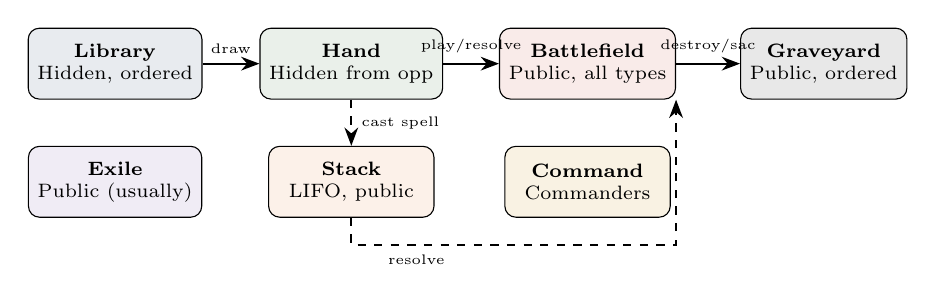
\begin{tikzpicture}[
      every node/.style={font=\scriptsize},
      zone/.style={draw, rounded corners, fill=#1,
                   minimum width=2.1cm, minimum height=0.9cm, align=center},
      >=Stealth,
    ]
    \node[zone=mtgblue!10]   (lib)  at (0, 0)     {\textbf{Library}\\Hidden, ordered};
    \node[zone=mtggreen!10]  (hand) at (3, 0)     {\textbf{Hand}\\Hidden from opp};
    \node[zone=mtgred!10]    (bf)   at (6, 0)     {\textbf{Battlefield}\\Public, all types};
    \node[zone=lgray]        (gy)   at (9, 0)     {\textbf{Graveyard}\\Public, ordered};
    \node[zone=kgpurple!10]  (ex)   at (0, -1.5)  {\textbf{Exile}\\Public (usually)};
    \node[zone=jepaorange!10](stk)  at (3, -1.5)  {\textbf{Stack}\\LIFO, public};
    \node[zone=mtggold!15]   (cmd)  at (6, -1.5)  {\textbf{Command}\\Commanders};

    \draw[->, thick] (lib) -- (hand) node[midway, above, font=\tiny] {draw};
    \draw[->, thick] (hand) -- (bf) node[midway, above, font=\tiny] {play/resolve};
    \draw[->, thick] (bf) -- (gy) node[midway, above, font=\tiny] {destroy/sac};
    \draw[->, thick, dashed] (hand.south) -- ++(0,-0.3) -| (stk.north)
      node[pos=0.25, right, font=\tiny] {cast spell};
    \draw[->, thick, dashed] (stk) -- ++(0,-0.8) -| (bf.south east)
      node[pos=0.1, below, font=\tiny] {resolve};
  \end{tikzpicture}
  \end{center}
  \vspace{0.2cm}
  \footnotesize
  Zone transitions are the \textbf{atoms of gameplay}: every action is a zone change.\\
  The tokenizer encodes each zone separately (hand: 10$\times$128, battlefield: 20$\times$128$+$4, graveyard: 20$\times$128, stack: 5$\times$130).
\end{frame}

% --- Slide: Abilities & Effects ------------------------------------
\begin{frame}{Abilities, Triggers \& Continuous Effects}
  \begin{columns}[T]
    \begin{column}{0.48\textwidth}
      \footnotesize
      \textbf{Activated abilities:}
      \begin{itemize}\scriptsize
        \item Parsed from oracle text via regex: ``\{cost\}: effect''
        \item Mana ability detection (produces mana $\to$ no stack)
        \item Zone, controller, tap cost checks
        \item Effects: add mana, draw, gain life, deal damage, discard
      \end{itemize}
      \vspace{0.15cm}
      \textbf{Triggered abilities:}
      \begin{itemize}\scriptsize
        \item TriggerEvent enum: ETB, attacks, spell\_cast, turn\_begins, \ldots
        \item \texttt{detect\_enters\_battlefield()} scans state diffs
        \item Triggers go on stack, obey priority
      \end{itemize}
    \end{column}
    \begin{column}{0.48\textwidth}
      \footnotesize
      \textbf{Continuous effects (CR 611 layers):}
      \begin{itemize}\scriptsize
        \item 10 layers applied in order by timestamp
        \item Layer 4: type changes
        \item Layer 6: ability granting/removal
        \item Layer 7a/b: power/toughness setting/modification
        \item \texttt{ContinuousEffectRegistry} sorts (layer, timestamp)
      \end{itemize}
      \vspace{0.15cm}
      \textbf{Keywords supported (25 in v1.1):}\\
      {\scriptsize Flying, First Strike, Double Strike, Deathtouch, Trample,
       Haste, Flash, Hexproof, Lifelink, Menace, Vigilance, Reach,
       Indestructible, Ward, Defender, Shroud, Cycling, Kicker, \ldots}\\
      {\scriptsize Target: extract 475+ remaining via LLM agents.}
    \end{column}
  \end{columns}
\end{frame}

% --- Slide: Combat System ------------------------------------------
\begin{frame}{Combat System}
  \begin{center}
  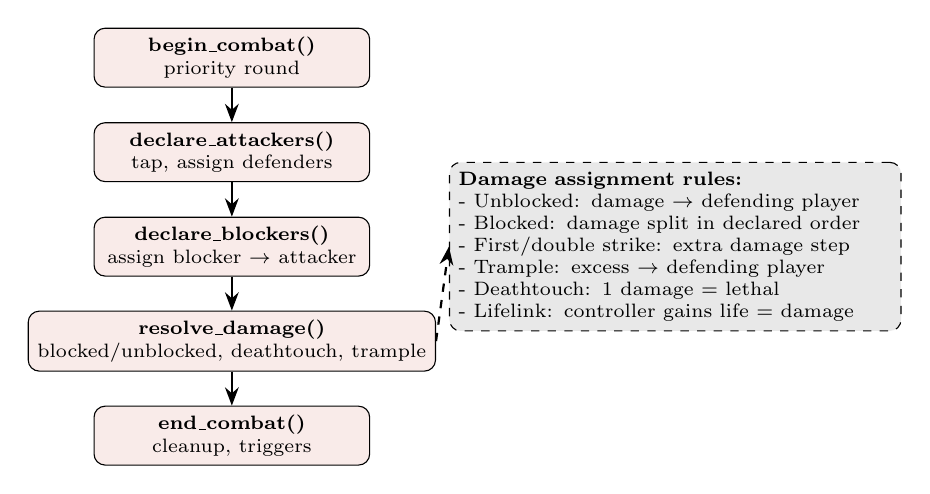
\begin{tikzpicture}[
      every node/.style={font=\scriptsize},
      sbox/.style={draw, rounded corners, fill=mtgred!10,
                  minimum width=3.5cm, minimum height=0.7cm, align=center},
      >=Stealth,
    ]
    \node[sbox] (s1) at (0, 2)    {\textbf{begin\_combat()}\\priority round};
    \node[sbox] (s2) at (0, 0.8)  {\textbf{declare\_attackers()}\\tap, assign defenders};
    \node[sbox] (s3) at (0, -0.4) {\textbf{declare\_blockers()}\\assign blocker $\to$ attacker};
    \node[sbox] (s4) at (0, -1.6) {\textbf{resolve\_damage()}\\blocked/unblocked, deathtouch, trample};
    \node[sbox] (s5) at (0, -2.8) {\textbf{end\_combat()}\\cleanup, triggers};

    \draw[->, thick] (s1) -- (s2);
    \draw[->, thick] (s2) -- (s3);
    \draw[->, thick] (s3) -- (s4);
    \draw[->, thick] (s4) -- (s5);

    \node[draw, dashed, rounded corners, fill=lgray,
          text width=5.5cm, align=left, font=\scriptsize,
          right=1cm of s3] (det)
      {\textbf{Damage assignment rules:}\\
       - Unblocked: damage $\to$ defending player\\
       - Blocked: damage split in declared order\\
       - First/double strike: extra damage step\\
       - Trample: excess $\to$ defending player\\
       - Deathtouch: 1 damage = lethal\\
       - Lifelink: controller gains life = damage};
    \draw[->, dashed, thick] (s4.east) -- (det.west);
  \end{tikzpicture}
  \end{center}
\end{frame}


% ===================================================================
\section{Agent System}
% ===================================================================

% --- Slide: Agent Zoo Overview -------------------------------------
\begin{frame}{The Agent Zoo: 7 Architectures}
  \begin{center}
  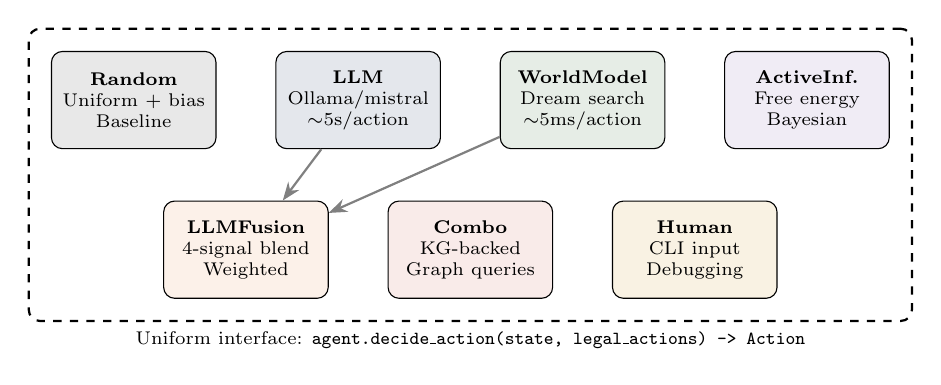
\begin{tikzpicture}[
      every node/.style={font=\scriptsize},
      agent/.style={draw, rounded corners, minimum width=2.2cm,
                    minimum height=1.3cm, align=center},
      >=Stealth, scale=0.95, transform shape,
    ]
    \node[agent, fill=lgray]         (rand) at (0, 0)
      {\textbf{Random}\\Uniform + bias\\Baseline};
    \node[agent, fill=mtgblue!12]    (llm)  at (3, 0)
      {\textbf{LLM}\\Ollama/mistral\\$\sim$5s/action};
    \node[agent, fill=mtggreen!12]   (wm)   at (6, 0)
      {\textbf{WorldModel}\\Dream search\\$\sim$5ms/action};
    \node[agent, fill=kgpurple!10]   (ai)   at (9, 0)
      {\textbf{ActiveInf.}\\Free energy\\Bayesian};
    \node[agent, fill=jepaorange!10] (fus)  at (1.5, -2)
      {\textbf{LLMFusion}\\4-signal blend\\Weighted};
    \node[agent, fill=mtgred!10]     (cmb)  at (4.5, -2)
      {\textbf{Combo}\\KG-backed\\Graph queries};
    \node[agent, fill=mtggold!15]    (hum)  at (7.5, -2)
      {\textbf{Human}\\CLI input\\Debugging};

    \node[draw, thick, dashed, rounded corners,
          fit=(rand)(llm)(wm)(ai)(fus)(cmb)(hum),
          inner sep=8pt,
          label={[font=\scriptsize]below:Uniform interface:
            \texttt{agent.decide\_action(state, legal\_actions) -> Action}}] {};

    \draw[->, thick, gray] (llm) -- (fus);
    \draw[->, thick, gray] (wm)  -- (fus);
  \end{tikzpicture}
  \end{center}
  \vspace{0.1cm}
  \begin{center}\footnotesize
    Any agent vs.\ any agent $\Rightarrow$ tournaments, ELO ratings, architecture A/B tests.
  \end{center}
\end{frame}

% --- Slide: LLM Agent Details --------------------------------------
\begin{frame}{LLM Agent: Ollama Integration}
  \begin{columns}[T]
    \begin{column}{0.52\textwidth}
      \footnotesize
      \textbf{Setup:}
      \begin{itemize}\scriptsize
        \item Ollama at \texttt{localhost:11434}
        \item Models: mistral (default), phi, llama2, neural-chat
        \item Temperature: 0.2 (consistency)
        \item Timeout: 10s HTTP, 30s generate
        \item Auto fallback to RandomAgent
      \end{itemize}
      \vspace{0.2cm}
      \textbf{Prompt construction:}
      \begin{itemize}\scriptsize
        \item System prompt: 5 decision factors (mana efficiency, board presence, life, card advantage, tempo)
        \item Context: game state, hand, creatures, lands, opponent board
        \item Legal actions grouped by type priority
        \item Parse: extract integer index from response
      \end{itemize}
    \end{column}
    \begin{column}{0.45\textwidth}
      \footnotesize
      \textbf{LLMFusion --- 4-signal blend:}
      \vspace{0.2cm}
      \begin{center}
      \begin{tabular}{@{}lc@{}}
        \toprule
        \textbf{Signal} & \textbf{Weight} \\
        \midrule
        World Model (dream EV) & 0.40 \\
        LLM (strategic pref.)  & 0.30 \\
        Heuristic (board eval)  & 0.15 \\
        KG (combo/synergy)      & 0.15 \\
        \bottomrule
      \end{tabular}
      \end{center}
      \vspace{0.2cm}
      \scriptsize
      LLM skipped if one action dominates ($>$0.8).\\
      Dream config: 8 rollouts $\times$ depth 10, $\tau = 1.15$.\\
      Lazy initialization of sub-components.
    \end{column}
  \end{columns}
\end{frame}

% --- Slide: Active Inference Agent ---------------------------------
\begin{frame}{Active Inference Agent: Free Energy Principle}
  \begin{columns}[T]
    \begin{column}{0.55\textwidth}
      \footnotesize
      \textbf{Expected Free Energy:}
      $$G(\pi) = -\underbrace{\text{epistemic}}_{\text{information gain}} - \underbrace{\text{pragmatic}}_{\text{goal achievement}}$$

      \textbf{Epistemic values} (info-gathering actions):
      \begin{itemize}\scriptsize
        \item Reveal/discard effects $\to$ 0.40
        \item Sacrifice + hand peek $\to$ 0.35
        \item Draw card $\to$ 0.20
      \end{itemize}
      \vspace{0.15cm}
      \textbf{Pragmatic values} (goal-achieving actions):
      \begin{itemize}\scriptsize
        \item Win/infinite combo $\to$ 0.50
        \item Creature: power / 20 (capped 0.4)
        \item Removal spell $\to$ 0.25
        \item Ramp spell $\to$ 0.15
        \item Generic: CMC / 10 (capped 0.3)
      \end{itemize}
    \end{column}
    \begin{column}{0.42\textwidth}
      \footnotesize
      \textbf{Bayesian belief updates:}
      \begin{itemize}\scriptsize
        \item Opponent archetype distribution updated each observation
        \item Blue mana $\geq 2$ open $\to$ $+$0.15 P(counterspell), cap 0.95
        \item Should\_hold\_open\_mana(): instants vs.\ opponent threats
      \end{itemize}
      \vspace{0.2cm}
      \textbf{Decision flow:}
      \begin{enumerate}\scriptsize
        \item Observe game state
        \item Update beliefs (Bayesian)
        \item Score all actions by $G(\pi)$
        \item Sort: lower $G$ = better
        \item Pick argmin
      \end{enumerate}
    \end{column}
  \end{columns}
\end{frame}

% --- Slide: Opponent Modeling --------------------------------------
\begin{frame}{Opponent Modeling: Bayesian + Hypergeometric}
  \begin{columns}[T]
    \begin{column}{0.55\textwidth}
      \footnotesize
      \textbf{With known decklist:}
      \begin{itemize}\scriptsize
        \item Track: copies\_in\_deck, copies\_seen, copies\_drawn, copies\_remaining
        \item Hypergeometric draw probability:
          $$P(\geq 1 \mid N, k_0, k) = 1 - \frac{\binom{N-k_0}{k}}{\binom{N}{k}}$$
        \item Exact P(counterspell), P(removal), P(boardwipe) each draw
        \item Process-of-elimination as cards are revealed
      \end{itemize}
      \vspace{0.2cm}
      \textbf{Without decklist:}
      \begin{itemize}\scriptsize
        \item Archetype inference from observed plays
        \item Archetype-based staple card predictions
        \item More spells than attacks $\to$ P(control/combo) higher
        \item Default P(counterspell) = 0.15
      \end{itemize}
    \end{column}
    \begin{column}{0.42\textwidth}
      \footnotesize
      \textbf{ThreatAssessment output:}
      \begin{itemize}\scriptsize
        \item archetype + confidence
        \item predicted\_hand (top-$k$ cards)
        \item P(counterspell)
        \item P(removal)
        \item P(boardwipe)
        \item cards\_remaining\_in\_deck
        \item cards\_in\_hand\_count
      \end{itemize}
      \vspace{0.15cm}
      \textbf{Behavior tracking:}
      \begin{itemize}\scriptsize
        \item observe\_card(name, zone)
        \item observe\_card\_played(name)
        \item observe\_behavior(action, state)
        \item Playstyle ratio: spell/attack
      \end{itemize}
    \end{column}
  \end{columns}
\end{frame}


% ===================================================================
\section{World Model (V+M+C)}
% ===================================================================

% --- Slide: V+M+C Overview ----------------------------------------
\begin{frame}{World Model: Ha \& Schmidhuber (2018) for Card Games}
  \begin{center}
  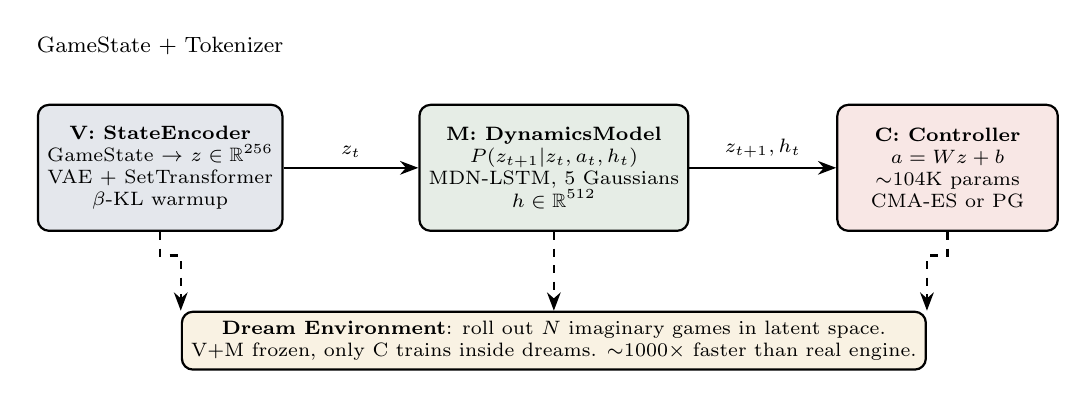
\begin{tikzpicture}[
      every node/.style={font=\scriptsize},
      block/.style={draw, thick, rounded corners, minimum width=2.8cm,
                    minimum height=1.6cm, align=center},
      >=Stealth,
    ]
    \node[block, fill=mtgblue!12] (V) at (0,0)
      {\textbf{V: StateEncoder}\\GameState $\to$ $z \in \mathbb{R}^{256}$\\VAE + SetTransformer\\$\beta$-KL warmup};
    \node[block, fill=mtggreen!12] (M) at (5,0)
      {\textbf{M: DynamicsModel}\\$P(z_{t+1} | z_t, a_t, h_t)$\\MDN-LSTM, 5 Gaussians\\$h \in \mathbb{R}^{512}$};
    \node[block, fill=mtgred!12] (C) at (10,0)
      {\textbf{C: Controller}\\$a = Wz + b$\\$\sim$104K params\\CMA-ES or PG};

    \node[above=0.5cm of V, font=\footnotesize] {GameState + Tokenizer};
    \draw[->, thick] (V) -- (M) node[midway, above] {$z_t$};
    \draw[->, thick] (M) -- (C) node[midway, above] {$z_{t+1}, h_t$};

    \node[draw, thick, rounded corners, fill=mtggold!15,
          minimum width=7cm, align=center, below=1cm of M] (dream)
      {\textbf{Dream Environment}: roll out $N$ imaginary games in latent space.\\
       V+M frozen, only C trains inside dreams. $\sim$1000$\times$ faster than real engine.};

    \draw[->, thick, dashed] (V.south) -- ++(0,-0.3) -| (dream.north west);
    \draw[->, thick, dashed] (M.south) -- (dream.north);
    \draw[->, thick, dashed] (C.south) -- ++(0,-0.3) -| (dream.north east);
  \end{tikzpicture}
  \end{center}
\end{frame}

% --- Slide: State Encoder details ----------------------------------
\begin{frame}{V: StateEncoder --- VAE with SetEncoder}
  \begin{columns}[T]
    \begin{column}{0.55\textwidth}
      \footnotesize
      \textbf{GameTokenizer output:}
      \begin{center}
      \begin{tabular}{@{}llr@{}}
        \toprule
        \textbf{Feature} & \textbf{Shape} & \textbf{Dim} \\
        \midrule
        player\_features   & (12,)       & 12 \\
        opponent\_features  & (12,)       & 12 \\
        hand\_cards         & (10, 128)   & 1280 \\
        battlefield\_cards  & (20, 128+4) & 2640 \\
        opp\_battlefield    & (20, 128)   & 2560 \\
        graveyard\_cards    & (20, 128)   & 2560 \\
        stack\_features     & (5, 130)    & 650 \\
        phase + turn        & (16,)       & 16 \\
        \bottomrule
      \end{tabular}
      \end{center}
    \end{column}
    \begin{column}{0.42\textwidth}
      \footnotesize
      \textbf{Architecture:}
      \begin{enumerate}\scriptsize
        \item SetEncoder per zone: MLP per card $+$ masked mean pooling (permutation-invariant)
        \item Zone outputs: hand/$\frac{h}{4}$, battlefield/$\frac{h}{4}$+4, opp/$\frac{h}{4}$, gy/$\frac{h}{8}$, stack/$\frac{h}{8}$+2
        \item Player: 11 feats $\times$ 2 $\to$ $\frac{h}{4}$
        \item Phase: 12 one-hot + 4 turn $\to$ $\frac{h}{8}$
        \item Concat $\to$ MLP $\to$ fused
        \item Optional: $+$ kg\_proj(KG embed)
        \item VAE bottleneck: $\mu, \log\sigma^2$
        \item Reparameterize: $z = \mu + \sigma \cdot \epsilon$
      \end{enumerate}
      \vspace{0.1cm}
      \textbf{Loss:} MSE(reconstruct) $+ \beta \cdot$ KL\\
      $\beta$ warmup: 0 $\to$ 0.001 over 10 epochs
    \end{column}
  \end{columns}
\end{frame}

% --- Slide: Dynamics Model -----------------------------------------
\begin{frame}{M: MDN-LSTM --- Predicting the Future}
  \begin{columns}[T]
    \begin{column}{0.5\textwidth}
      \footnotesize
      \textbf{Input:} $[z_t; a_t] \in \mathbb{R}^{256+136}$
      \begin{itemize}\scriptsize
        \item Action encoding: 8 one-hot type + 128-d card embed = 136
        \item 2-layer LSTM, hidden $h \in \mathbb{R}^{512}$
        \item Optional: 4-layer Transformer (8 heads, max seq 200)
      \end{itemize}
      \vspace{0.15cm}
      \textbf{MDN Head} (Mixture Density Network):
      \begin{itemize}\scriptsize
        \item $K = 5$ Gaussian components
        \item Outputs: $\pi_k$ (mixing), $\mu_k$ ($K \times 256$), $\sigma_k$ ($K \times 256$)
        \item Log-sigma clamped $[-7, 2]$
        \item Sample: Categorical($\pi$) $\to$ Gaussian($\mu_k, \sigma_k$)
      \end{itemize}
    \end{column}
    \begin{column}{0.47\textwidth}
      \footnotesize
      \textbf{Additional heads:}
      \begin{itemize}\scriptsize
        \item Done head: $\sigma(\text{linear}(h)) \to P(\text{game over})$
        \item Reward head: linear$(h) \to \hat{r}_t$
      \end{itemize}
      \vspace{0.15cm}
      \textbf{Training loss:}
      $$\mathcal{L}_M = -\log\sum_k \pi_k \, \mathcal{N}(z_{t+1}; \mu_k, \sigma_k)$$
      $$+ \text{BCE}(\hat{d}, d) + \text{MSE}(\hat{r}, r)$$
      \vspace{0.15cm}
      \textbf{Dream temperature $\tau$:}\\
      Default 1.15 (harder dreams).\\
      Dreams explore more diverse futures than reality.\\
      Controller learns robustness from harder scenarios.
    \end{column}
  \end{columns}
\end{frame}

% --- Slide: Controller ---------------------------------------------
\begin{frame}{C: Controller --- Minimal Brain, Maximum Speed}
  \begin{columns}[T]
    \begin{column}{0.5\textwidth}
      \footnotesize
      \textbf{Architecture:}\\
      $a = W \cdot [z; h] + b$
      \begin{itemize}\scriptsize
        \item Linear: $(256 + 512) \times 136 = \sim$104K params
        \item Optional MLP: + hidden layer (64-d, Tanh)
        \item Dot-product scoring against encoded legal actions
        \item Masked softmax $\to$ log-probabilities
      \end{itemize}
      \vspace{0.15cm}
      \textbf{CMA-ES training:}
      \begin{itemize}\scriptsize
        \item Population: 64 parameter vectors
        \item Each evaluated over 16 dream rollouts
        \item 100 generations
        \item \texttt{get\_flat\_params() / set\_flat\_params()}
      \end{itemize}
    \end{column}
    \begin{column}{0.47\textwidth}
      \footnotesize
      \textbf{Policy Gradient alternative:}
      \begin{itemize}\scriptsize
        \item REINFORCE with baseline
        \item lr = 3e-4, grad clip = 1.0
        \item Checkpoint: \texttt{controller\_pg\_final.pt}
      \end{itemize}
      \vspace{0.15cm}
      \textbf{Dream search (inference):}
      \begin{itemize}\scriptsize
        \item For each legal action $a_i$:
        \item Roll out 8 $\times$ 10-step futures
        \item Score: cumulative discounted reward ($\gamma = 0.99$)
        \item Pick $\arg\max_i \text{avg}(\text{scores}_i)$
        \item MCTS-like in latent space
      \end{itemize}
      \vspace{0.15cm}
      \textbf{Key}: V and M are frozen during C training.\\
      Controller trains \textit{entirely inside dreams}.
    \end{column}
  \end{columns}
\end{frame}


% ===================================================================
\section{Knowledge Graph}
% ===================================================================

% --- Slide: KG Overview -------------------------------------------
\begin{frame}{Knowledge Graph: Neo4j + OWL + SHACL}
  \begin{columns}[T]
    \begin{column}{0.55\textwidth}
      \footnotesize
      \textbf{Technology:}
      \begin{itemize}\scriptsize
        \item Neo4j 5 Community Edition
        \item n10s plugin: OWL ontology import
        \item APOC plugin: graph algorithms, path expansion
        \item Ports: 7474 (browser) / 7687 (bolt)
      \end{itemize}
      \vspace{0.15cm}
      \textbf{Node labels:}
      \begin{itemize}\scriptsize
        \item \textbf{Card}: 28,000+ from Scryfall (name, type, cost, oracle text, P/T)
        \item \textbf{Combo}: 10,000+ from Commander Spellbook
        \item \textbf{Archetype}: aggro, control, combo, midrange, tempo
        \item \textbf{Keyword}: 25 modeled (475+ remaining)
        \item \textbf{Effect}: damage, draw, counter, ramp, removal
      \end{itemize}
    \end{column}
    \begin{column}{0.42\textwidth}
      \footnotesize
      \textbf{Relationships:}
      \begin{itemize}\scriptsize
        \item PART\_OF\_COMBO
        \item SYNERGIZES\_WITH
        \item COUNTERS
        \item ENABLES
        \item HAS\_KEYWORD
        \item BELONGS\_TO\_ARCHETYPE
      \end{itemize}
      \vspace{0.15cm}
      \textbf{Key queries:}
      \begin{itemize}\scriptsize
        \item detect\_available\_combos(cards)
        \item detect\_near\_combos(cards)
        \item infer\_archetype(seen\_cards)
        \item get\_synergies\_for(card)
      \end{itemize}
    \end{column}
  \end{columns}
\end{frame}

% --- Slide: OWL Ontology ------------------------------------------
\begin{frame}[fragile]{OWL Ontology: 4-Layer Design}
  \begin{center}
  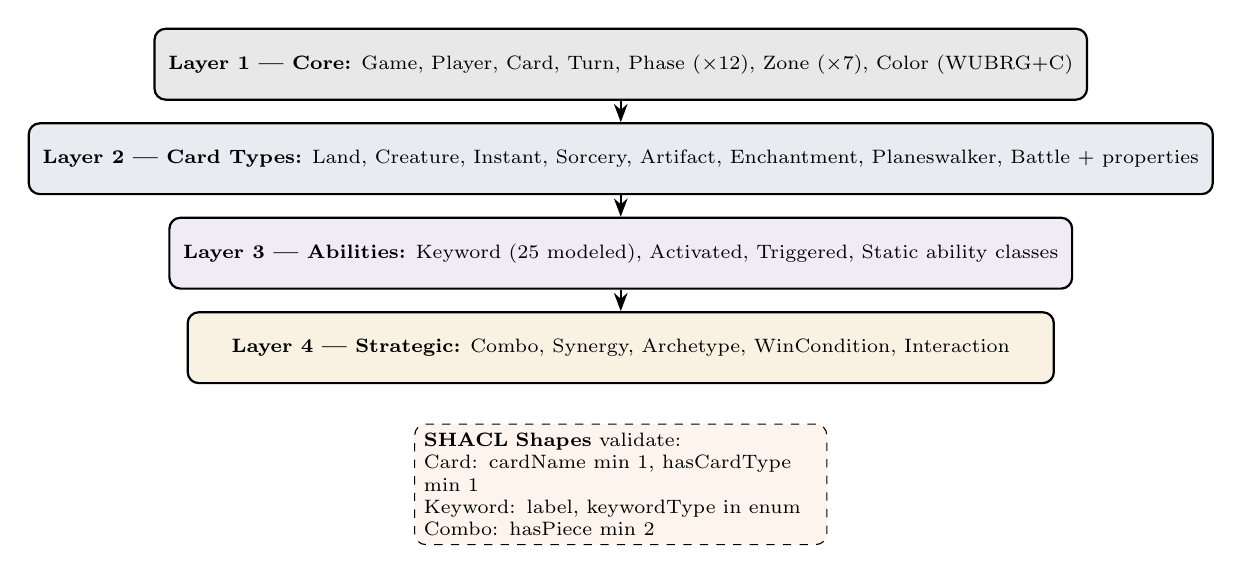
\begin{tikzpicture}[
      every node/.style={font=\scriptsize},
      layer/.style={draw, thick, rounded corners, fill=#1,
                    minimum width=11cm, minimum height=0.9cm, align=left, inner sep=5pt},
      >=Stealth,
    ]
    \node[layer=lgray] (l1) at (0, 3)
      {\textbf{Layer 1 --- Core:} Game, Player, Card, Turn, Phase ($\times$12), Zone ($\times$7), Color (WUBRG+C)};
    \node[layer=mtgblue!10] (l2) at (0, 1.8)
      {\textbf{Layer 2 --- Card Types:} Land, Creature, Instant, Sorcery, Artifact, Enchantment, Planeswalker, Battle + properties};
    \node[layer=kgpurple!10] (l3) at (0, 0.6)
      {\textbf{Layer 3 --- Abilities:} Keyword (25 modeled), Activated, Triggered, Static ability classes};
    \node[layer=mtggold!15] (l4) at (0, -0.6)
      {\textbf{Layer 4 --- Strategic:} Combo, Synergy, Archetype, WinCondition, Interaction};

    \draw[->, thick] (l1) -- (l2);
    \draw[->, thick] (l2) -- (l3);
    \draw[->, thick] (l3) -- (l4);

    \node[draw, dashed, rounded corners, text width=5cm, align=left,
          font=\scriptsize, fill=jepaorange!8, below=0.5cm of l4] (shacl)
      {\textbf{SHACL Shapes} validate:\\
       Card: cardName min 1, hasCardType min 1\\
       Keyword: label, keywordType in enum\\
       Combo: hasPiece min 2};
  \end{tikzpicture}
  \end{center}
  \vspace{0.1cm}
  \begin{center}\footnotesize
    Namespace: \texttt{http://purl.org/mtg/ontology\#}\\
    Current: $\sim$1000 lines. Target: $\sim$5000 lines (5$\times$ expansion via LLM agents).
  \end{center}
\end{frame}

% --- Slide: KG Import Pipeline ------------------------------------
\begin{frame}[fragile]{KG Pipeline: Scryfall $\to$ GraphSAGE $\to$ Neo4j}
  \begin{center}
  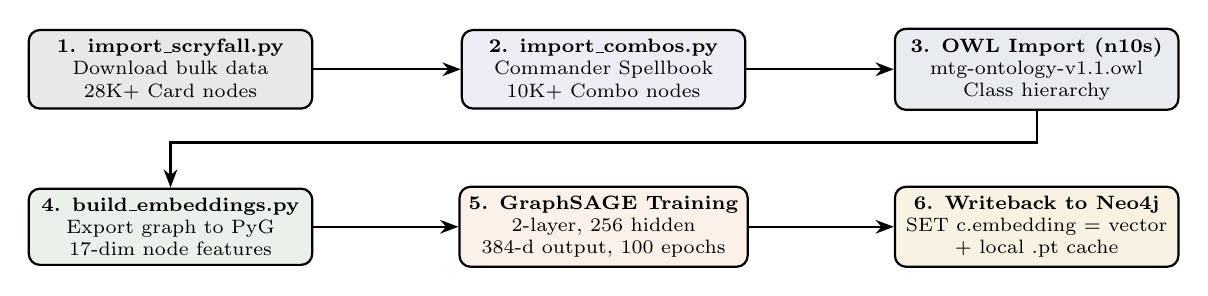
\begin{tikzpicture}[
      every node/.style={font=\scriptsize},
      sbox/.style={draw, thick, rounded corners, fill=#1,
                   minimum width=3.6cm, minimum height=0.9cm, align=center},
      >=Stealth,
    ]
    \node[sbox=lgray]        (s1) at (0, 2)
      {\textbf{1. import\_scryfall.py}\\Download bulk data\\28K+ Card nodes};
    \node[sbox=kgpurple!10]  (s2) at (5.5, 2)
      {\textbf{2. import\_combos.py}\\Commander Spellbook\\10K+ Combo nodes};
    \node[sbox=mtgblue!10]   (s3) at (11, 2)
      {\textbf{3. OWL Import (n10s)}\\mtg-ontology-v1.1.owl\\Class hierarchy};

    \node[sbox=mtggreen!10]  (s4) at (0, 0)
      {\textbf{4. build\_embeddings.py}\\Export graph to PyG\\17-dim node features};
    \node[sbox=jepaorange!10](s5) at (5.5, 0)
      {\textbf{5. GraphSAGE Training}\\2-layer, 256 hidden\\384-d output, 100 epochs};
    \node[sbox=mtggold!15]   (s6) at (11, 0)
      {\textbf{6. Writeback to Neo4j}\\SET c.embedding = vector\\+ local .pt cache};

    \draw[->, thick] (s1) -- (s2);
    \draw[->, thick] (s2) -- (s3);
    \draw[->, thick] (s3.south) -- ++(0,-0.4) -| (s4.north);
    \draw[->, thick] (s4) -- (s5);
    \draw[->, thick] (s5) -- (s6);
  \end{tikzpicture}
  \end{center}
  \vspace{0.2cm}
  \begin{center}
  \footnotesize
  \textbf{Graph RAG} (6 retrieval strategies): subgraph (APOC path expansion),
  Cypher (LLM-generated), vector (Neo4j native index),
  fulltext (Lucene), community (Louvain), hybrid (RRF fusion).
  \end{center}
\end{frame}


% ===================================================================
\section{JEPA Integration}
% ===================================================================

% --- Slide: What is JEPA / LeWM -----------------------------------
\begin{frame}{JEPA / LeWM: Predict in Latent Space, Not Pixel Space}
  \footnotesize
  \textbf{Paper:} Maes et al.\ (2026), ``LeWorldModel: Stable End-to-End JEPA from Pixels,''
  arXiv:2603.19312\\
  \textbf{JEPA} = Joint Embedding Predictive Architecture (LeCun 2022)
  \vspace{0.3cm}
  \begin{center}
  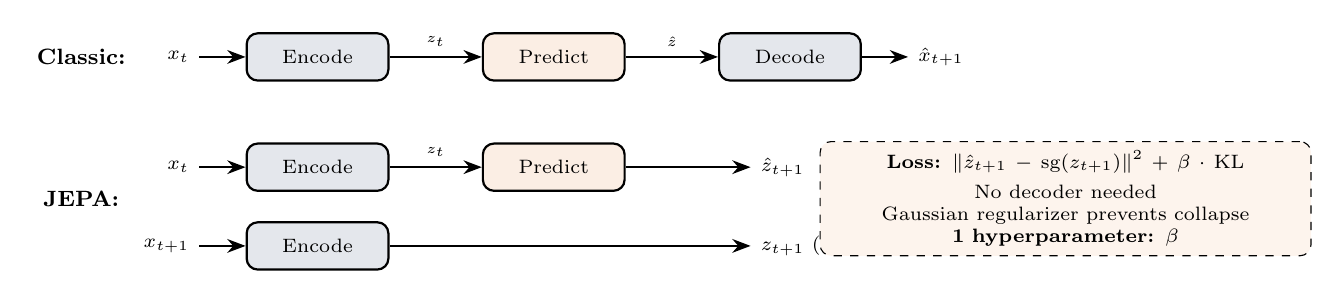
\begin{tikzpicture}[
      every node/.style={font=\scriptsize},
      enc/.style={draw, thick, rounded corners, fill=mtgblue!12,
                  minimum width=1.8cm, minimum height=0.6cm, align=center},
      pred/.style={draw, thick, rounded corners, fill=jepaorange!12,
                   minimum width=1.8cm, minimum height=0.6cm, align=center},
      >=Stealth,
    ]
    \node[font=\footnotesize\bfseries] at (-1.5, 1.8) {Classic:};
    \node[enc]  (e1) at (1.5, 1.8)  {Encode};
    \node[pred] (p1) at (4.5, 1.8)  {Predict};
    \node[enc]  (d1) at (7.5, 1.8)  {Decode};
    \draw[->, thick] (0, 1.8) node[left] {$x_t$} -- (e1);
    \draw[->, thick] (e1) -- (p1) node[midway, above, font=\tiny] {$z_t$};
    \draw[->, thick] (p1) -- (d1) node[midway, above, font=\tiny] {$\hat{z}$};
    \draw[->, thick] (d1) -- (9, 1.8) node[right] {$\hat{x}_{t+1}$};

    \node[font=\footnotesize\bfseries] at (-1.5, 0) {JEPA:};
    \node[enc]  (e2) at (1.5, 0.4)   {Encode};
    \node[pred] (p2) at (4.5, 0.4)   {Predict};
    \node[enc]  (e3) at (1.5, -0.6)  {Encode};
    \draw[->, thick] (0, 0.4)  node[left] {$x_t$}     -- (e2);
    \draw[->, thick] (e2) -- (p2) node[midway, above, font=\tiny] {$z_t$};
    \draw[->, thick] (p2) -- (7, 0.4) node[right] {$\hat{z}_{t+1}$};
    \draw[->, thick] (0, -0.6) node[left] {$x_{t+1}$} -- (e3);
    \draw[->, thick] (e3) -- (7, -0.6) node[right] {$z_{t+1}$ (target)};

    \node[draw, dashed, rounded corners, fill=jepaorange!8,
          text width=6cm, align=center, font=\scriptsize]
      at (11, 0)
      {\textbf{Loss:} $\|\hat{z}_{t+1} - \text{sg}(z_{t+1})\|^2 + \beta \cdot \text{KL}$\\[3pt]
       No decoder needed\\
       Gaussian regularizer prevents collapse\\
       \textbf{1 hyperparameter:} $\beta$};
  \end{tikzpicture}
  \end{center}
\end{frame}

% --- Slide: JEPA vs DIAMOND Numbers -------------------------------
\begin{frame}{LeWM Numbers That Matter}
  \begin{center}
  \begin{tabular}{@{}lccc@{}}
    \toprule
    \textbf{Metric} & \textbf{LeWM} & \textbf{Foundation WM} & \textbf{DIAMOND} \\
    \midrule
    Parameters       & $\sim$15M     & $\sim$1B+              & 4.4--381M \\
    Training         & 1 GPU, hours  & Multi-GPU, days        & Multi-GPU, days \\
    Planning speed   & Baseline      & \textbf{48$\times$ slower}  & Faster \\
    Loss terms       & \textbf{2}    & 6--8                   & 3--4 \\
    Hyperparameters  & \textbf{1}    & 5--7                   & 3--5 \\
    Collapse avoidance & Gaussian reg. & EMA + stop-grad     & VQ-VAE \\
    Latent structure & \textbf{Semantic} & Unclear            & Discrete tokens \\
    \bottomrule
  \end{tabular}
  \end{center}
  \vspace{0.3cm}
  \begin{center}
  \footnotesize
  \textbf{Why JEPA for MTG:}\\
  Game state is structured data, not pixels.  JEPA predicts in latent space directly.\\
  Gaussian regularizer encodes semantic structure (mana, life, cards) --- confirmed by probing.\\
  48$\times$ faster planning $\Rightarrow$ more rollouts per turn.
  \end{center}
\end{frame}

% --- Slide: Dual-Input Architecture --------------------------------
\begin{frame}{Dual-Input JEPA Architecture}
  \begin{center}
  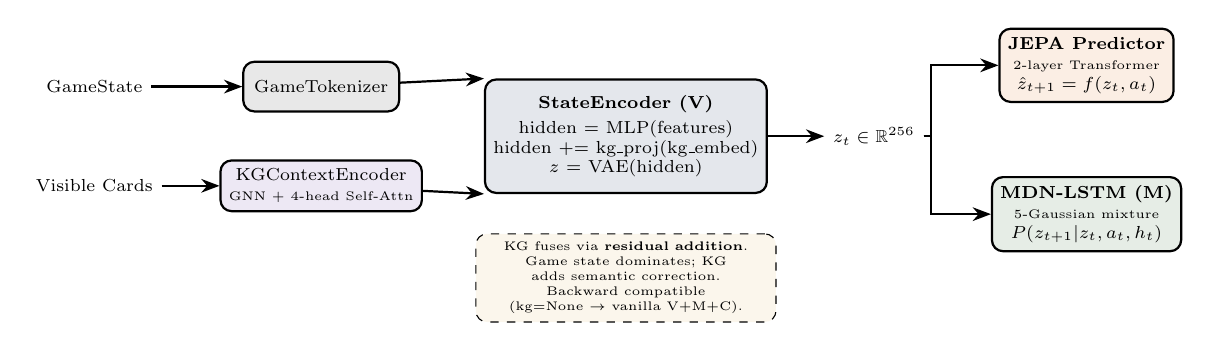
\begin{tikzpicture}[
      every node/.style={font=\scriptsize},
      block/.style={draw, thick, rounded corners, minimum height=0.7cm, align=center},
      >=Stealth, scale=0.9, transform shape,
    ]
    \node (gs) at (-2, 3)   {GameState};
    \node (vc) at (-2, 1.6) {Visible Cards};

    \node[block, fill=lgray, minimum width=2.2cm] (tok) at (1.2, 3)
      {GameTokenizer};
    \draw[->, thick] (gs) -- (tok);

    \node[block, fill=kgpurple!12, minimum width=2.2cm] (kge) at (1.2, 1.6)
      {KGContextEncoder\\{\tiny GNN + 4-head Self-Attn}};
    \draw[->, thick] (vc) -- (kge);

    \node[block, fill=mtgblue!12, minimum width=3.5cm,
          minimum height=1.6cm] (enc) at (5.5, 2.3)
      {\textbf{StateEncoder (V)}\\[2pt]
       hidden = MLP(features)\\
       hidden += kg\_proj(kg\_embed)\\
       $z$ = VAE(hidden)};
    \draw[->, thick] (tok) -- (enc.north west);
    \draw[->, thick] (kge) -- (enc.south west);

    \node (zt) at (9, 2.3) {$z_t \in \mathbb{R}^{256}$};
    \draw[->, thick] (enc) -- (zt);

    \node[block, fill=jepaorange!12, minimum width=2.3cm,
          minimum height=1cm] (jepa) at (12, 3.3)
      {\textbf{JEPA Predictor}\\{\tiny 2-layer Transformer}\\
       $\hat{z}_{t+1} = f(z_t, a_t)$};

    \node[block, fill=mtggreen!12, minimum width=2.3cm,
          minimum height=1cm] (mdn) at (12, 1.2)
      {\textbf{MDN-LSTM (M)}\\{\tiny 5-Gaussian mixture}\\
       $P(z_{t+1} | z_t, a_t, h_t)$};

    \draw[->, thick] (zt) -- ++(0.8,0) |- (jepa.west);
    \draw[->, thick] (zt) -- ++(0.8,0) |- (mdn.west);

    \node[draw, dashed, rounded corners, fill=mtggold!10,
          text width=4cm, font=\tiny, align=center]
      at (5.5, 0.3)
      {KG fuses via \textbf{residual addition}.\\
       Game state dominates; KG adds semantic correction.\\
       Backward compatible (kg=None $\to$ vanilla V+M+C).};
  \end{tikzpicture}
  \end{center}
\end{frame}

% --- Slide: JEPA Loss & Surprise ----------------------------------
\begin{frame}{JEPA Training \& Surprise Detection}
  \begin{columns}[T]
    \begin{column}{0.48\textwidth}
      \footnotesize
      \textbf{JEPA Loss (2 terms):}
      $$\mathcal{L} = \underbrace{\|\hat{z}_{t+1} - \text{sg}(z_{t+1})\|^2}_{\text{prediction}}
        + \beta \cdot \underbrace{\text{KL}(q(z) \| \mathcal{N}(0,I))}_{\text{regularizer}}$$
      \begin{itemize}\scriptsize
        \item Stop-gradient on target $z_{t+1}$ (no collapse)
        \item $\beta = 1.0$ (single hyperparameter)
        \item 2-layer pre-norm Transformer encoder
        \item Input: project($[z_t; a_t]$) $\to$ $\mathbb{R}^{512}$
        \item Output: project $\to$ $\hat{z}_{t+1} \in \mathbb{R}^{256}$
      \end{itemize}
    \end{column}
    \begin{column}{0.48\textwidth}
      \footnotesize
      \textbf{Surprise detection:}
      $$S = \|\hat{z}_{t+1} - z_{\text{actual}}\|^2$$
      \begin{itemize}\scriptsize
        \item High $S$: observed transition was ``implausible''
        \item 4/4 survives Bolt? $\to$ KG: ``Indestructible''
        \item Opponent gains 20 life? $\to$ KG: ``Storm combo''
        \item \textbf{Self-correcting:} surprise flags KG gaps
      \end{itemize}
      \vspace{0.2cm}
      \textbf{Dual paths at inference:}
      \begin{itemize}\scriptsize
        \item MDN-LSTM: stochastic, sequential $h$
        \item JEPA: deterministic, single-step
        \item Agent uses MDN for dreams, JEPA for fast eval
      \end{itemize}
    \end{column}
  \end{columns}
\end{frame}


% ===================================================================
\section{Training Pipeline}
% ===================================================================

% --- Slide: 6-Stage Pipeline --------------------------------------
\begin{frame}[fragile]{Training: 6-Stage Pipeline}
  \begin{center}
  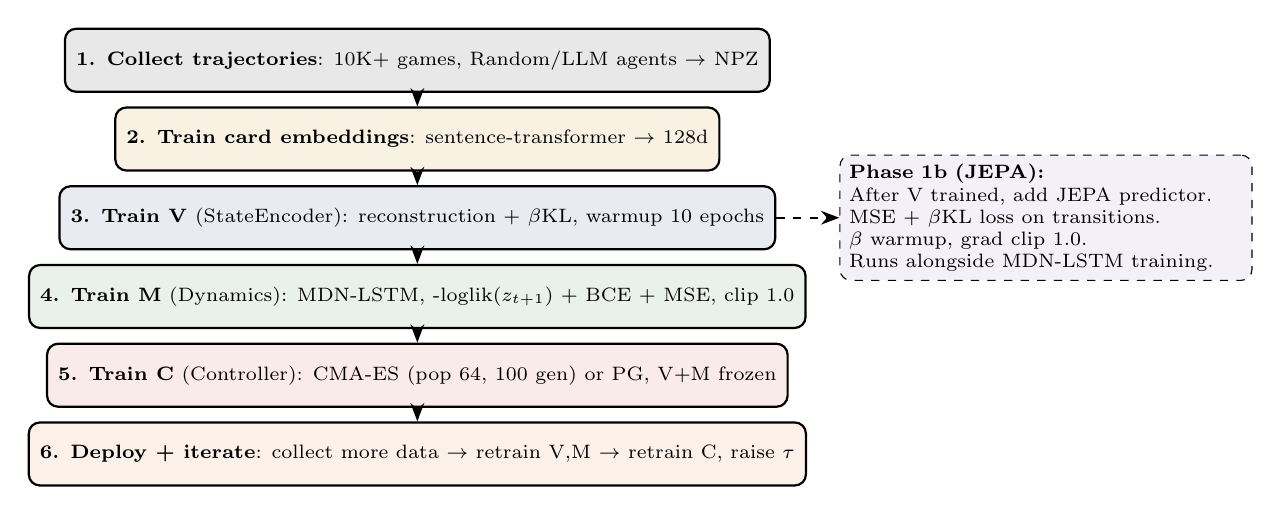
\begin{tikzpicture}[
      every node/.style={font=\scriptsize},
      stage/.style={draw, thick, rounded corners, fill=#1,
                    minimum width=5.5cm, minimum height=0.8cm, align=left, inner sep=4pt},
      >=Stealth,
    ]
    \node[stage=lgray]          (s1) at (0, 3.6)
      {\textbf{1. Collect trajectories}:
       10K+ games, Random/LLM agents $\to$ NPZ};
    \node[stage=mtggold!15]     (s2) at (0, 2.6)
      {\textbf{2. Train card embeddings}:
       sentence-transformer $\to$ 128d};
    \node[stage=mtgblue!10]     (s3) at (0, 1.6)
      {\textbf{3. Train V} (StateEncoder):
       reconstruction + $\beta$KL, warmup 10 epochs};
    \node[stage=mtggreen!10]    (s4) at (0, 0.6)
      {\textbf{4. Train M} (Dynamics):
       MDN-LSTM, -loglik($z_{t+1}$) + BCE + MSE, clip 1.0};
    \node[stage=mtgred!10]      (s5) at (0, -0.4)
      {\textbf{5. Train C} (Controller):
       CMA-ES (pop 64, 100 gen) or PG, V+M frozen};
    \node[stage=jepaorange!10]  (s6) at (0, -1.4)
      {\textbf{6. Deploy + iterate}:
       collect more data $\to$ retrain V,M $\to$ retrain C, raise $\tau$};

    \draw[->, thick] (s1) -- (s2);
    \draw[->, thick] (s2) -- (s3);
    \draw[->, thick] (s3) -- (s4);
    \draw[->, thick] (s4) -- (s5);
    \draw[->, thick] (s5) -- (s6);

    \node[draw, dashed, rounded corners, fill=kgpurple!8,
          text width=5cm, align=left, font=\scriptsize,
          right=0.8cm of s3] (jepar)
      {\textbf{Phase 1b (JEPA):}\\
       After V trained, add JEPA predictor.\\
       MSE + $\beta$KL loss on transitions.\\
       $\beta$ warmup, grad clip 1.0.\\
       Runs alongside MDN-LSTM training.};
    \draw[->, dashed, thick] (s3.east) -- (jepar.west);
  \end{tikzpicture}
  \end{center}
\end{frame}

% --- Slide: Transfer Learning --------------------------------------
\begin{frame}[fragile]{Transfer Learning: Standard $\to$ Commander}
  \begin{center}
  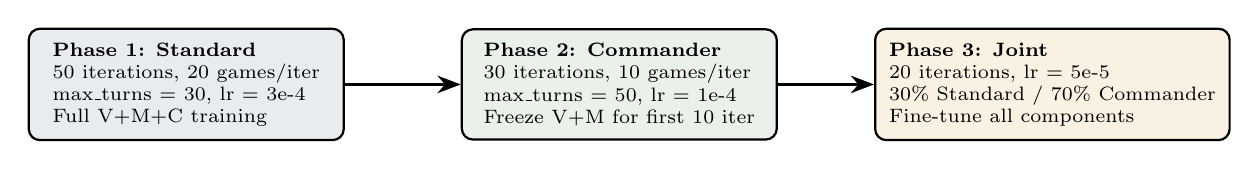
\begin{tikzpicture}[
      every node/.style={font=\scriptsize},
      phase/.style={draw, thick, rounded corners, fill=#1,
                    minimum width=4cm, minimum height=1.4cm, align=left, inner sep=5pt},
      >=Stealth,
    ]
    \node[phase=mtgblue!10] (p1) at (0, 0)
      {\textbf{Phase 1: Standard}\\50 iterations, 20 games/iter\\max\_turns = 30, lr = 3e-4\\Full V+M+C training};
    \node[phase=mtggreen!10] (p2) at (5.5, 0)
      {\textbf{Phase 2: Commander}\\30 iterations, 10 games/iter\\max\_turns = 50, lr = 1e-4\\Freeze V+M for first 10 iter};
    \node[phase=mtggold!15] (p3) at (11, 0)
      {\textbf{Phase 3: Joint}\\20 iterations, lr = 5e-5\\30\% Standard / 70\% Commander\\Fine-tune all components};

    \draw[->, very thick] (p1) -- (p2);
    \draw[->, very thick] (p2) -- (p3);
  \end{tikzpicture}
  \end{center}
  \vspace{0.4cm}
  \begin{columns}[T]
    \begin{column}{0.48\textwidth}
      \footnotesize
      \textbf{Reward function:}
      \begin{itemize}\scriptsize
        \item Terminal: $+$1.0 win, $-$1.0 loss
        \item Life delta: $\Delta L \times 0.01/40$
        \item Card advantage: $\Delta C \times 0.005$
        \item Board presence: $\Delta B \times 0.005$
        \item Per-action penalty: $-$0.001
      \end{itemize}
    \end{column}
    \begin{column}{0.48\textwidth}
      \footnotesize
      \textbf{Self-play (AlphaZero-style):}
      \begin{itemize}\scriptsize
        \item 64 parallel games
        \item 100K experience buffer
        \item Batch 256, 10 epochs
        \item lr = 1e-4
        \item 100 eval games per iteration
      \end{itemize}
    \end{column}
  \end{columns}
\end{frame}


% ===================================================================
\section{LangGraph Orchestrator}
% ===================================================================

% --- Slide: LangGraph Game Graph -----------------------------------
\begin{frame}[fragile]{LangGraph Orchestrator: Phase-Driven Game Loop}
  \begin{center}
  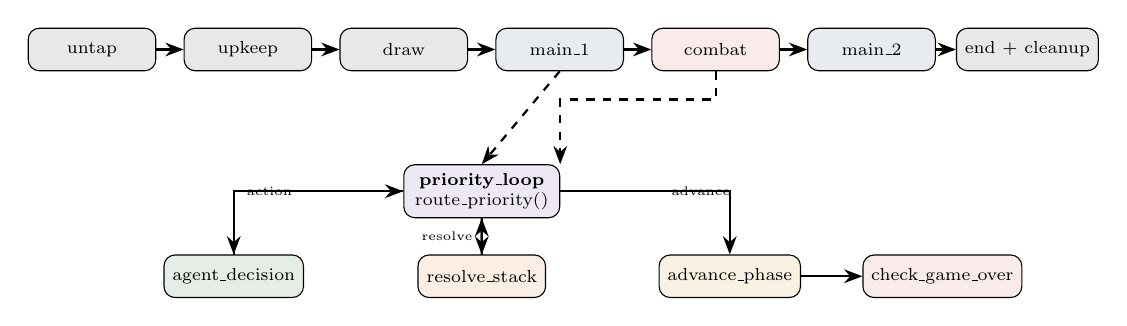
\begin{tikzpicture}[
      every node/.style={font=\scriptsize},
      node/.style={draw, rounded corners, fill=#1,
                   minimum width=1.8cm, minimum height=0.6cm, align=center},
      >=Stealth, scale=0.9, transform shape,
    ]
    % Phase nodes
    \node[node=lgray]        (untap)   at (0, 2)     {untap};
    \node[node=lgray]        (upkeep)  at (2.2, 2)   {upkeep};
    \node[node=lgray]        (draw)    at (4.4, 2)   {draw};
    \node[node=mtgblue!10]   (main1)   at (6.6, 2)   {main\_1};
    \node[node=mtgred!10]    (combat)  at (8.8, 2)   {combat};
    \node[node=mtgblue!10]   (main2)   at (11, 2)    {main\_2};
    \node[node=lgray]        (end)     at (13.2, 2)  {end + cleanup};

    % Priority loop
    \node[node=kgpurple!12, minimum width=2.2cm] (ploop) at (5.5, 0)
      {\textbf{priority\_loop}\\route\_priority()};
    \node[node=mtggreen!12]  (agent) at (2, -1.2)
      {agent\_decision};
    \node[node=jepaorange!12](resolve) at (5.5, -1.2)
      {resolve\_stack};
    \node[node=mtggold!15]   (advance) at (9, -1.2)
      {advance\_phase};
    \node[node=mtgred!10]    (gameover) at (12, -1.2)
      {check\_game\_over};

    % Connections
    \draw[->, thick] (untap) -- (upkeep);
    \draw[->, thick] (upkeep) -- (draw);
    \draw[->, thick] (draw) -- (main1);
    \draw[->, thick] (main1) -- (combat);
    \draw[->, thick] (combat) -- (main2);
    \draw[->, thick] (main2) -- (end);

    \draw[->, thick, dashed] (main1.south) -- (ploop.north);
    \draw[->, thick, dashed] (combat.south) -- ++(0,-0.4) -| (ploop.north east);

    % Priority routing
    \draw[->, thick] (ploop) -| (agent)
      node[pos=0.3, left, font=\tiny] {action};
    \draw[->, thick] (ploop) -- (resolve)
      node[midway, left, font=\tiny] {resolve};
    \draw[->, thick] (ploop) -| (advance)
      node[pos=0.3, right, font=\tiny] {advance};

    \draw[->, thick] (agent) |- (ploop);
    \draw[->, thick] (resolve) -- ++(0, 0.6) -- (ploop);
    \draw[->, thick] (advance) -- (gameover);
  \end{tikzpicture}
  \end{center}
  \vspace{0.15cm}
  \begin{center}\footnotesize
    \textbf{route\_priority()}: all passed + stack non-empty $\to$ resolve;
    all passed + empty $\to$ advance; else $\to$ agent\_decision.\\
    APNAP order enforced. Supports multiplayer Commander.
  \end{center}
\end{frame}


% ===================================================================
\section{Deployment}
% ===================================================================

% --- Slide: Docker -------------------------------------------------
\begin{frame}{Docker Deployment}
  \begin{columns}[T]
    \begin{column}{0.48\textwidth}
      \footnotesize
      \textbf{docker-compose.yml} (local):
      \begin{itemize}\scriptsize
        \item \textbf{neo4j}: Neo4j 5, n10s + APOC, 7474/7687
        \item Heap: 512m--1G, PageCache: 512m
        \item Volumes: data, logs, ontology
      \end{itemize}
      \vspace{0.2cm}
      \textbf{docker-compose.remote.yml} (GPU):
      \begin{itemize}\scriptsize
        \item \textbf{ollama}: ollama/ollama:latest, GPU passthrough (nvidia, all GPUs), port 11434
        \item \textbf{trainer}: Python + GPU, depends on neo4j + ollama
        \item \textbf{jepa-trainer}: JEPA-specific training entry
        \item Neo4j: 2--4G heap, 2G pagecache
      \end{itemize}
    \end{column}
    \begin{column}{0.48\textwidth}
      \footnotesize
      \textbf{Dockerfile:}
      \begin{itemize}\scriptsize
        \item Python 3.12-slim base
        \item 3 requirements files:\\
              \texttt{requirements.txt} (core)\\
              \texttt{requirements-ml.txt} (torch, PyG)\\
              \texttt{requirements-ontology.txt} (rdflib, owlrl)
        \item Copies: src/, scripts/, data/, neo4j/
        \item Entrypoint: \texttt{python scripts/deploy.py}
      \end{itemize}
      \vspace{0.2cm}
      \textbf{deploy.py orchestration:}
      \begin{enumerate}\scriptsize
        \item check\_infrastructure()
        \item build\_knowledge\_graph()
        \item run\_rl\_training()
        \item run\_dream\_training()
        \item play\_demo\_game()
      \end{enumerate}
    \end{column}
  \end{columns}
\end{frame}


% ===================================================================
\section{Key Numbers \& Testing}
% ===================================================================

% --- Slide: Key Numbers --------------------------------------------
\begin{frame}{Key Numbers At a Glance}
  \begin{center}
  \begin{tabular}{@{}lr@{\quad}lr@{}}
    \toprule
    \textbf{Component} & \textbf{Value} & \textbf{Component} & \textbf{Value} \\
    \midrule
    Latent dim $z$       & 256        & Dream rollouts        & 8 \\
    Card embedding       & 128-d      & Dream depth           & 10 steps \\
    LSTM hidden $h$      & 512        & Dream max             & 50 steps \\
    Action encoding      & 136        & Dream temp $\tau$     & 1.15 \\
    MDN components       & 5          & CMA-ES population     & 64 \\
    Controller params    & $\sim$104K & CMA-ES generations    & 100 \\
    V+M params           & $\sim$2--5M & RL learning rate     & 3e-4 \\
    JEPA Transformer     & 2L, 4H, 512 & Self-play batch     & 256 \\
    JEPA $\beta$         & 1.0        & Experience buffer     & 100K \\
    KG attention heads   & 4          & Scryfall cards        & 28K+ \\
    GraphSAGE output     & 384-d      & Combos imported       & 10K+ \\
    Max hand/bf/gy       & 10/20/20   & OWL keywords          & 25 / 500+ \\
    Discount $\gamma$    & 0.99       & Fusion: WM/LLM/H/KG  & .40/.30/.15/.15 \\
    \bottomrule
  \end{tabular}
  \end{center}
\end{frame}

% --- Slide: Testing ------------------------------------------------
\begin{frame}{Testing: 28 Test Files}
  \begin{columns}[T]
    \begin{column}{0.32\textwidth}
      \footnotesize
      \textbf{Engine tests:}
      \begin{itemize}\scriptsize
        \item test\_game\_engine
        \item test\_game\_execution
        \item test\_game\_simulator
        \item test\_combat\_game
        \item test\_combat\_debug
        \item test\_stack\_priority
        \item test\_game\_scenarios
      \end{itemize}
    \end{column}
    \begin{column}{0.32\textwidth}
      \footnotesize
      \textbf{Ability tests:}
      \begin{itemize}\scriptsize
        \item test\_activated\_abilities
        \item test\_triggered\_abilities
        \item test\_triggered\_ability\_interactions
        \item test\_additional\_triggers
        \item test\_static\_abilities
        \item test\_ability\_integration
      \end{itemize}
    \end{column}
    \begin{column}{0.32\textwidth}
      \footnotesize
      \textbf{Agent / System tests:}
      \begin{itemize}\scriptsize
        \item test\_agent\_strategies
        \item test\_ollama\_agent
        \item test\_knowledge\_graph
        \item test\_world\_model\_pytest
        \item test\_end\_to\_end
        \item test\_end\_to\_end\_game
        \item test\_tournament
      \end{itemize}
    \end{column}
  \end{columns}
  \vspace{0.3cm}
  \begin{center}\footnotesize
    Run: \texttt{pytest tests/} or \texttt{pytest --cov=src tests/}\\
    Additional test directories: \texttt{tests/test\_agents/}, \texttt{tests/test\_engine/}, \texttt{tests/test\_knowledge/}
  \end{center}
\end{frame}


% ===================================================================
\section{Novelty \& Future Work}
% ===================================================================

% --- Slide: What's Novel ------------------------------------------
\begin{frame}{What Makes This Novel}
  \begin{center}
  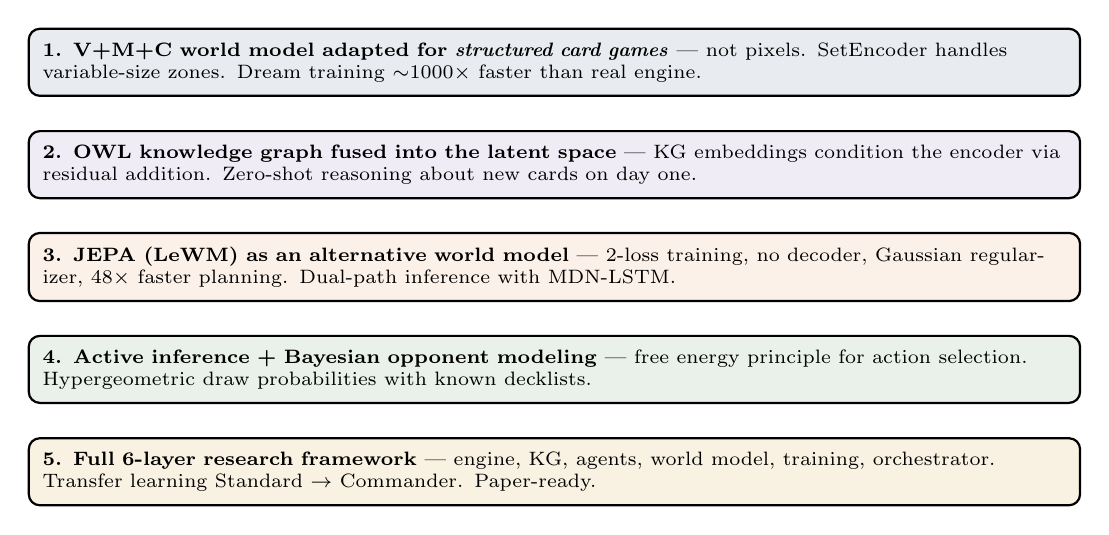
\begin{tikzpicture}[
      every node/.style={font=\scriptsize},
      item/.style={draw, thick, rounded corners, text width=13cm,
                   align=left, inner sep=5pt},
    ]
    \node[item, fill=mtgblue!10] at (0, 3.5)
      {\textbf{1. V+M+C world model adapted for \textit{structured card games}}
       --- not pixels. SetEncoder handles variable-size zones.
       Dream training $\sim$1000$\times$ faster than real engine.};
    \node[item, fill=kgpurple!10] at (0, 2.2)
      {\textbf{2. OWL knowledge graph fused into the latent space}
       --- KG embeddings condition the encoder via residual addition.
       Zero-shot reasoning about new cards on day one.};
    \node[item, fill=jepaorange!10] at (0, 0.9)
      {\textbf{3. JEPA (LeWM) as an alternative world model}
       --- 2-loss training, no decoder, Gaussian regularizer,
       48$\times$ faster planning. Dual-path inference with MDN-LSTM.};
    \node[item, fill=mtggreen!10] at (0, -0.4)
      {\textbf{4. Active inference + Bayesian opponent modeling}
       --- free energy principle for action selection.
       Hypergeometric draw probabilities with known decklists.};
    \node[item, fill=mtggold!15] at (0, -1.7)
      {\textbf{5. Full 6-layer research framework}
       --- engine, KG, agents, world model, training, orchestrator.
       Transfer learning Standard $\to$ Commander. Paper-ready.};
  \end{tikzpicture}
  \end{center}
\end{frame}

% --- Slide: Future Work -------------------------------------------
\begin{frame}{Future Work}
  \begin{columns}[T]
    \begin{column}{0.48\textwidth}
      \textbf{Short-term:}
      \begin{itemize}\small
        \item Benchmark WM+KG+JEPA vs.\ vanilla V+M+C
        \item Latent space probing (mana, life, card advantage)
        \item Dream speedup measurement
        \item GPU Docker training at scale
      \end{itemize}
      \vspace{0.3cm}
      \textbf{Medium-term:}
      \begin{itemize}\small
        \item Extract 475+ remaining keywords via LLM agents
        \item Multi-LLM ontology extension (HITL + SHACL)
        \item Tournament ELO system with real decklists
        \item Streamlit / Web UI visualization
      \end{itemize}
    \end{column}
    \begin{column}{0.48\textwidth}
      \textbf{Long-term:}
      \begin{itemize}\small
        \item Commander 4-player with alliance dynamics
        \item Deck construction agent (KG-guided)
        \item Cross-format transfer at scale
        \item Paper: ``Structured Imagination for Complex Card Games''
      \end{itemize}
      \vspace{0.3cm}
      \textbf{Research questions:}
      \begin{itemize}\small
        \item Does KG conditioning improve sample efficiency $10\times$?
        \item Can surprise detection close KG gaps automatically?
        \item Is JEPA's latent space more interpretable than MDN's?
      \end{itemize}
    \end{column}
  \end{columns}
\end{frame}


% ===================================================================
\section{Conclusion}
% ===================================================================

% --- Slide: Final Thesis ------------------------------------------
\begin{frame}{Final Thesis}
  \begin{center}
    \large\bfseries
    World Model + Knowledge Graph + JEPA + Active Inference\\
    = Structured Imagination for the Hardest Card Game
  \end{center}
  \vspace{0.3cm}
  \begin{center}
  \scalebox{0.8}{%
    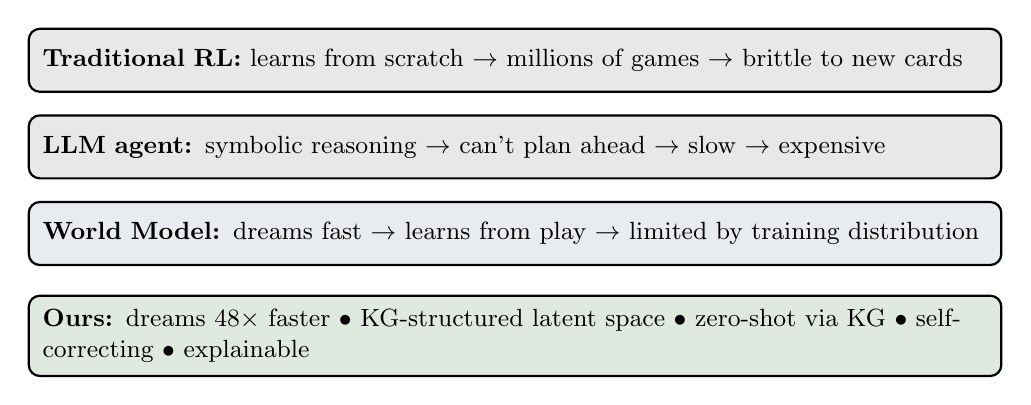
\begin{tikzpicture}[
        every node/.style={font=\small},
        row/.style={draw, thick, rounded corners, text width=12cm,
                    align=left, minimum height=0.8cm, inner sep=5pt},
      ]
      \node[row, fill=lgray] at (0, 2.2)
        {\textbf{Traditional RL:} learns from scratch $\to$ millions of games $\to$ brittle to new cards};
      \node[row, fill=lgray] at (0, 1.1)
        {\textbf{LLM agent:} symbolic reasoning $\to$ can't plan ahead $\to$ slow $\to$ expensive};
      \node[row, fill=mtgblue!10] at (0, 0)
        {\textbf{World Model:} dreams fast $\to$ learns from play $\to$ limited by training distribution};
      \node[row, fill=mtggreen!15] at (0, -1.3)
        {\textbf{Ours:} dreams 48$\times$ faster $\bullet$ KG-structured latent space
         $\bullet$ zero-shot via KG $\bullet$ self-correcting $\bullet$ explainable};
    \end{tikzpicture}
  }
  \end{center}
  \vspace{0.3cm}
  \begin{center}
    \textit{This is not LLM reasoning about cards.\\
    This is not pure RL grinding through games.\\
    This is \textbf{structured imagination} --- the way humans actually play.}
  \end{center}
\end{frame}

% --- References ----------------------------------------------------
\begin{frame}{References}
  \footnotesize
  \begin{itemize}
    \item Ha, D. \& Schmidhuber, J. (2018). ``World Models.'' \textit{worldmodels.github.io}
    \item Maes, Le~Lidec, Scieur, LeCun, Balestriero (2026).
          ``LeWorldModel: Stable End-to-End JEPA from Pixels.'' \textit{arXiv:2603.19312}
    \item LeCun, Y. (2022). ``A Path Towards Autonomous Machine Intelligence.''
    \item Alonso, Jelley et al.\ (2024). ``DIAMOND: Diffusion for World Modeling.''
          \textit{NeurIPS 2024 Spotlight}
    \item Friston, K. (2010). ``The Free-Energy Principle: A Unified Brain Theory?''
          \textit{Nature Reviews Neuroscience}
    \item Hamilton et al.\ (2017). ``Inductive Representation Learning on Large Graphs.''
          \textit{NeurIPS 2017} (GraphSAGE)
    \item Hansen et al.\ (2016). ``CMA-ES: A Stochastic Method for Optimization.''
    \item MTG Comprehensive Rules (2025). Wizards of the Coast.
  \end{itemize}
\end{frame}

\end{document}
